%% ------------------------------------------------------------------------- %%
\chapter{Introduction}
\label{cap:Introduction}

One of the most used data structures in computer science are dictionaries. Those need to suport the operations of inserting, finding and deleting an element. If you think about it, this is one of the most executed tasks in many softwares. For example, when you have the list of numbers you last called on your cell phone and you want to know for each phone number, what is the person associated with it. A dictionary perfoms the task of inserting for each phone number the name of the person. Then you can retrieve that information finding, for a phone number, who is the person associated with it.


\begin{figure}[h!]
  \centering
  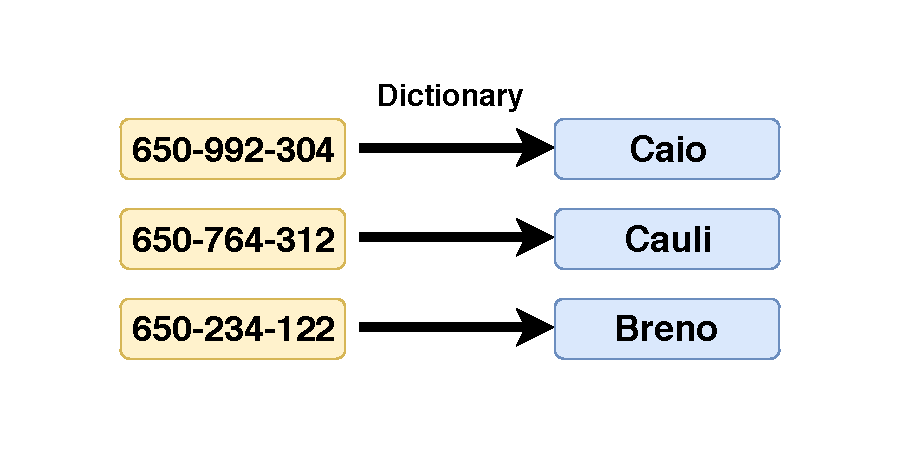
\includegraphics[width=12cm]{figuras/dictionary-example.pdf}
  \caption{Example of a dictionary that associates phone numbers to contact names. }
\end{figure}

Other use of a dictonary that we can think is to count the number of times you called a certain number. One of the most used implementation of dictionaries is with a hash table.

The implementation of a hash table always requires a hash function. This function usually takes the element that you want to hash, or key as it is usually called (In our example, the phone numbers), and ``digest'' it into a number. That number is then used to indentify the value (In our eaxmple, the contact names), in this structure that we call hash table.

An example of a hash function, that ``digest'' the phone numbers is the following: \\

\bigskip

\begin{figure}[h!]
  \centering
  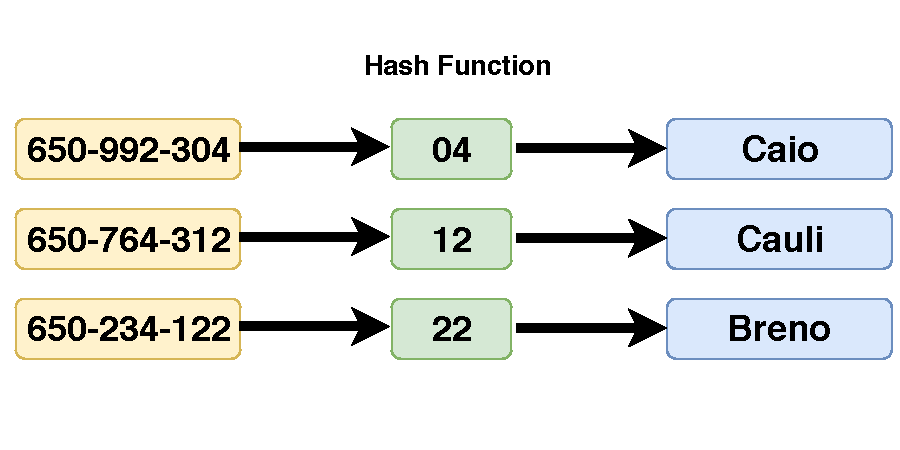
\includegraphics[width=12cm]{figuras/phone-hash-example.pdf}
  \caption{Example of a hash function hash function that just take the last 2 digits of the phone number }
\end{figure}

\medskip

As you can see this is a pretty simple function, it simply take the last 2 digits of each phone number. In this specific case, this is enough to uniquely identify each phone. We can imagine a function that can't uniquely identify each phone number, like getting just the last digit (in this case, Cauli's and Breno's numbers would have the same hash value), this will cause a collision in the table. Solving collisions in a hash table is a complete topic by itself, and it will be addressed in Chapter 3, Hash Tables. 

Solving collisions is actually a very important topic in hash tables, and that is because the vast majority of hash functions will have collisions. To picture that we can remember the ``Birthday Paradox'', that is the conclusion that we only need 23 people in a room to have a chance greater than \( 50\% \) of 2 or more people having the same birthday. In Donald Knuth's famous book, The Art of Computer Programming (Vol. 3, Chapter 6.4) \cite{TAOCP3}, he uses as an example a function from a 31-element set to a 41-element set, and from about \( 10^{50} \) functions only about \( 10^{43} \) give distinct values for each argument, that is about 1 in every 10 million functions. That shows that we will have collisions more often than not, so knowing how to deal with it is a major problem.

Hash functions and hash tables are among the most classic topics within computer science, yet is still one of the topics with most debate about what is state of the art. While the hash table was invented in 1953, widely discussed by Donald Knuth in his book, there are still many tweaks that can be made to boost its performance for specific use cases. One great example is F14, an open-source memory efficient hash table by Facebook \footnote{F14 is open sourced: \url{https://engineering.fb.com/developer-tools/f14/}}.

An example of lack of consensus in this area are the different hash functions and hash table implementations in different languages. There is no clear consensus on how to decide the size of a hash table, what are the tradeoffs of the collision-resolution algorithms or even what defines a good hash function. Hopefully, we got years of research on the topic to study and present a view on the subject, and that is what I am presenting thoughout this undegraduate thesis.

